\begin{figure}[H]
	\centering
	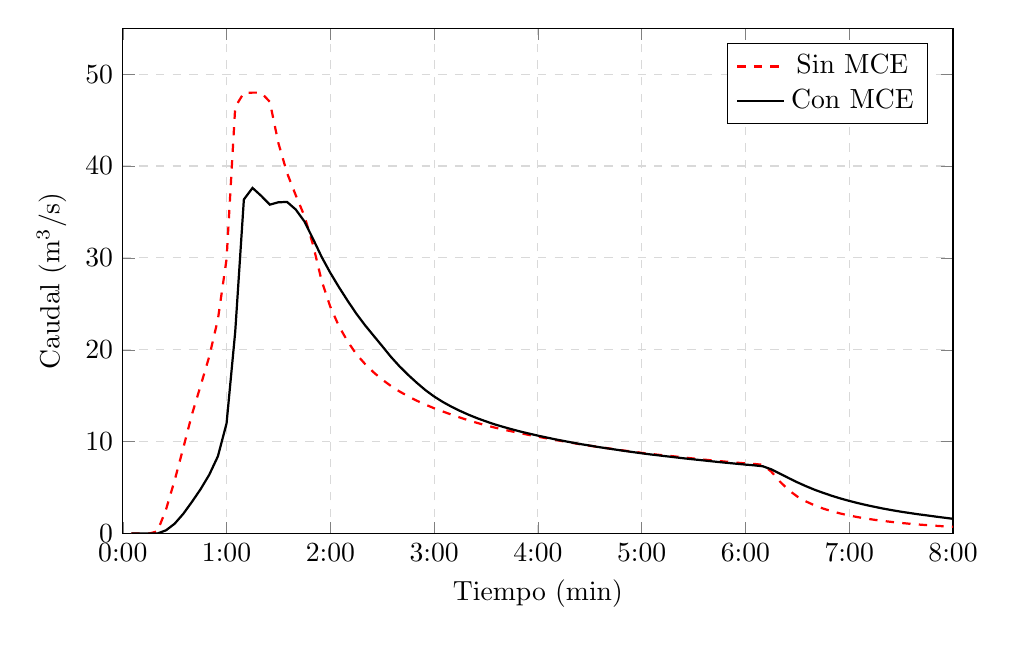
\begin{tikzpicture}
		\begin{axis}[
			width=\textwidth,
			height=8cm,
			xlabel={Tiempo (min)},
			ylabel={Caudal (m$^3$/s)},
			xmin=0,
			xmax=480,
			ymin=0,
			ymax=55,
			grid=major,
			grid style={dashed, gray!30},
			legend pos=north east,
			xtick={0, 60, 120, 180, 240, 300, 360, 420, 480},
			xticklabels={0:00, 1:00, 2:00, 3:00, 4:00, 5:00, 6:00, 7:00, 8:00},
			]
			% Sin MCE
			\addplot [
			red,
			thick,
			dashed,
			] coordinates {
				(5, 0.00) (10, 0.00) (15, 0.00) (20, 0.24) (25, 2.63)
				(30, 5.81) (35, 9.34) (40, 12.98) (45, 16.10) (50, 19.28)
				(55, 23.33) (60, 29.89) (65, 46.43) (70, 47.97) (75, 47.99)
				(80, 47.99) (85, 46.99) (90, 42.47) (95, 39.23) (100, 36.82)
				(105, 34.57) (110, 31.42) (115, 27.48) (120, 24.68) (125, 22.56)
				(130, 20.91) (135, 19.54) (140, 18.47) (145, 17.55) (150, 16.76)
				(155, 16.07) (160, 15.47) (165, 14.94) (170, 14.46) (175, 14.04)
				(180, 13.64) (185, 13.29) (190, 12.95) (195, 12.63) (200, 12.32)
				(205, 12.04) (210, 11.78) (215, 11.54) (220, 11.32) (225, 11.12)
				(230, 10.92) (235, 10.73) (240, 10.55) (245, 10.37) (250, 10.20)
				(255, 10.03) (260, 9.87) (265, 9.70) (270, 9.56) (275, 9.43)
				(280, 9.30) (285, 9.16) (290, 9.03) (295, 8.92) (300, 8.79)
				(305, 8.68) (310, 8.57) (315, 8.48) (320, 8.38) (325, 8.27)
				(330, 8.17) (335, 8.07) (340, 7.98) (345, 7.89) (350, 7.81)
				(355, 7.72) (360, 7.64) (365, 7.58) (370, 7.49) (375, 6.73)
				(380, 5.65) (385, 4.73) (390, 4.03) (395, 3.50) (400, 3.07)
				(405, 2.72) (410, 2.43) (415, 2.18) (420, 1.97) (425, 1.79)
				(430, 1.63) (435, 1.49) (440, 1.37) (445, 1.26) (450, 1.16)
				(455, 1.07) (460, 0.99) (465, 0.92) (470, 0.85) (475, 0.79)
				(480, 0.74)
			};
			\addlegendentry{Sin MCE}
			
			% Con MCE
			\addplot [
			black,
			thick,
			solid,
			] coordinates {
				(5, 0.00) (10, 0.00) (15, 0.00) (20, 0.01) (25, 0.36)
				(30, 1.08) (35, 2.16) (40, 3.46) (45, 4.84) (50, 6.41)
				(55, 8.42) (60, 12.00) (65, 21.96) (70, 36.36) (75, 37.62)
				(80, 36.76) (85, 35.80) (90, 36.06) (95, 36.09) (100, 35.27)
				(105, 33.97) (110, 32.07) (115, 30.10) (120, 28.37) (125, 26.81)
				(130, 25.34) (135, 23.94) (140, 22.69) (145, 21.54) (150, 20.40)
				(155, 19.24) (160, 18.20) (165, 17.27) (170, 16.41) (175, 15.61)
				(180, 14.92) (185, 14.33) (190, 13.81) (195, 13.35) (200, 12.93)
				(205, 12.55) (210, 12.21) (215, 11.89) (220, 11.61) (225, 11.35)
				(230, 11.10) (235, 10.88) (240, 10.66) (245, 10.46) (250, 10.26)
				(255, 10.08) (260, 9.90) (265, 9.73) (270, 9.58) (275, 9.42)
				(280, 9.28) (285, 9.14) (290, 9.00) (295, 8.87) (300, 8.74)
				(305, 8.62) (310, 8.51) (315, 8.40) (320, 8.29) (325, 8.18)
				(330, 8.08) (335, 7.98) (340, 7.88) (345, 7.78) (350, 7.69)
				(355, 7.60) (360, 7.51) (365, 7.43) (370, 7.33) (375, 6.99)
				(380, 6.52) (385, 6.04) (390, 5.58) (395, 5.16) (400, 4.77)
				(405, 4.43) (410, 4.11) (415, 3.82) (420, 3.56) (425, 3.32)
				(430, 3.10) (435, 2.90) (440, 2.71) (445, 2.54) (450, 2.38)
				(455, 2.24) (460, 2.10) (465, 1.98) (470, 1.85) (475, 1.73)
				(480, 1.61)
			};
			\addlegendentry{Con MCE}
			
		\end{axis}
	\end{tikzpicture}
	\caption{Comparación de hidrogramas en el punto de cierre de la cuenca con y sin medidas de control.}
	\label{fig:hidrograma_salida_comparacion}
\end{figure}
